\documentclass[11pt]{article}
\usepackage[T1]{fontenc}
\usepackage[margin=1in]{geometry}
\usepackage{amsmath,booktabs,graphicx,float,longtable,pdflscape,hyperref}
\title{Experiment 05 --- Spectral Lag and Latent-Proxy Corrections}
\author{Two-Layer CTMC experimental framework}
\date{FINAL ANALYSIS --- PRESPECIFIED 100-REPLICATION SAMPLE}
\begin{document}
\maketitle
\begin{center}\fbox{\textbf{FINAL ANALYSIS --- PRESPECIFIED 100-REPLICATION SAMPLE}}\end{center}

\begin{abstract}
This experiment tests two candidate aggregate-descriptor corrections to premature
inter-community leakage in MicroMacro simulation.  A spectral lag delays source
contagiousness, while a latent-boundary proxy relaxes toward aggregate prevalence.
Full Micro is the reference and all five variants share the network and initial
condition within a replication.  Inference uses the replication as the independent
unit and distinguishes completed-only Wasserstein metrics from censoring-aware
all-run RMST metrics.  The present document reports the final stage.
The analysis uses the prespecified replication IDs 1--100 for every scenario and variant.
\end{abstract}

\section{Research question}
Can spectral lag, latent-proxy relaxation, or their combination reduce sparse
chain-of-cliques terminal-arrival bias without knowing bridge-node identities?

\section{Motivation}
Section 3.7 of \emph{Notes on Micro--Macro Epidemic Networks} reports premature
leakage in the sparse benchmark. Experiment 01 separated hazard and placement
effects but left bridge-specific error. The corrections tested here are
\emph{candidate corrections proposed within the experimental framework, motivated
by spectral epidemic-threshold bounds}; they are not attributed to the article.

\section{Experimental design}
The five paired variants are V0 Full Micro, V1 production aggregate MicroMacro,
V2 lag-shifted MicroMacro, V3 latent-proxy MicroMacro, and V4 combined.
The baseline has $L=10$, $n=100$, $k=5$, mean internal degree approximately 6,
$\beta_{in}=\beta_{out}=0.003$, $\gamma=0$, $\tau_{micro}=1$, and
$T_{end}=4000$. Mini-sweeps vary $k\in\{1,5,10\}$ and
$d\in\{4,6,10\}$ without taking a Cartesian product. Network and initialization
streams are shared within replication; event streams are variant-specific. This is
a matched block design, not pathwise common-random-number pairing.

\section{Mathematical definitions}
For community $i$, $N_i$ is its size, $i_i(t)$ its infected count,
$\bar i_i(t)=i_i(t)/N_i$, and $\bar s_j(t)$ is normalized susceptibility.
The reference macro hazard is
\[\lambda^{ref}_{ij}(t)=\beta_{out}W_{ij}\bar i_i(t)\bar s_j(t).\]
The lag is
\[\tau_{find}(i)=\frac{\ln N_i}{\beta_{in}(\lambda_1(G_i)-1)},\qquad
  \bar i_i^{lag}(t)=\bar i_i(\max(0,t-\tau_{find}(i))),\]
and $\lambda^A_{ij}=\beta_{out}W_{ij}\bar i_i^{lag}\bar s_j$.
The latent rate and analytical synchronization update are
\[\kappa(i)=\frac{\beta_{in}(\lambda_1(G_i)-1)}{\ell(G_i)},\qquad
\bar i_i^B(t+\tau)=\bar i_i^B(t)+(1-e^{-\kappa(i)\tau})
  (\bar i_i(t)-\bar i_i^B(t)),\]
with $\bar i_i^B(0)=0$ and $\lambda^B_{ij}=\beta_{out}W_{ij}\bar i_i^B\bar s_j$.
V4 applies the same latent update to $\bar i_i^{lag}$. If $\lambda_1\le1$ or
$\ell$ is undefined, corrected outgoing hazard is zero and the descriptors are
flagged degenerate. Arrival definitions are $T_i=\inf\{t:i_i(t)>0\}$,
$T_{last}=T_{L-1}$, and $\Delta T_i=T_{i+1}-T_i$; censored values equal
$T_{end}$ with a separate observation flag.

\section{Parameters}
Each configured scenario uses a connected fixed-edge-count Erd\H{o}s--R\'enyi
community, uniform susceptible import placement, and one uniformly selected seed
in community zero. Graph descriptors are computed once before simulation.

\section{Implementation details}
Adjacency spectral radius is computed by shifted power iteration to tolerance
$10^{-6}$ with at most 1000 iterations and a residual-norm convergence check.
Mean shortest-path length is computed on the unweighted local graph. Lag history
uses fixed synchronization points and linear interpolation. The latent ODE uses
the analytical exponential update, not Euler integration. No descriptor fallback
is permitted. Outputs retain deterministic stream metadata and per-replication
graph checksums. Integrated hazard suppression measures how strongly each correction
changes V1 exposure, while synchronized correlation between $\bar i_i$ and the latent
state checks relaxation semantics. The proxy uses no boundary-node identities and
must not be interpreted as a direct bridge-aware state.

\section{Sanity checks}
\begin{table}[H]\centering
\caption{Recorded stage gates and actual diagnostic values.}
\begin{tabular}{p{.24\linewidth}p{.58\linewidth}p{.12\linewidth}}\toprule Gate & Value & Status \\\midrule
Historical reference & 20 archived replays; max arrival difference 4.55e-13 & passed \\ 
Formula and identity checks & descriptor ordering, degenerate case, scheduler identity, and zero-lag limit & passed \\ 
Final-sample integrity & 25 scenario-variant cells; replication IDs 1--100 present in every cell & passed \\ 
Schema and reproducibility & required columns present; recorded deterministic payload checks passed & passed \\ 
Production-code audit & before/after hashes identical; four pre-existing uncommitted file diffs & warning \\ 
\bottomrule\end{tabular}\end{table}
Interpretation below is conditional on the formula, reproducibility, pairing,
reference, schema, and production-immutability gates recorded in the manifest.
The production-immutability flag reflects pre-existing uncommitted production-code
changes: the recorded before/after hashes within this run are identical. It is an
audit warning, not evidence that the simulation changed its own code while running.

\section{Results tables}
Table 1 reports the primary all-run restricted $W_1$ and RMST metrics. The
completed-only relative $W_1$ is secondary and is shown only beside its completion
denominator. Baseline raw data also contain residual IDs above 100 from an older
interrupted launch; this report excludes them and uses IDs 1--100 uniformly.
\begin{landscape}
\scriptsize
\begin{longtable}{llrrrrr}
\toprule
Scenario & Variant & Completed & restricted $W_1$ [95\% CI] & completed rel. $W_1$ & $\Delta$RMST vs V0 [95\% CI] & $\Delta$RMST vs V1 \\
\midrule
\endfirsthead
\toprule
Scenario & Variant & Completed & restricted $W_1$ [95\% CI] & completed rel. $W_1$ & $\Delta$RMST vs V0 [95\% CI] & $\Delta$RMST vs V1 \\
\midrule
\endhead
baseline & Full Micro & 99/100 & 0 [0, 0] & 0 & 0 [0, 0] & -200.6 \\
baseline & Baseline MicroMacro & 98/100 & 208.2 [112.9, 319] & 0.06939 & 200.6 [98.16, 314.6] & 0 \\
baseline & Lag & 0/100 & 1071 [995.3, 1146] & NA & 1071 [993, 1151] & 870.3 \\
baseline & Latent proxy & 44/100 & 905.8 [816.9, 998.7] & 0.2421 & 905.8 [813.7, 992.6] & 705.2 \\
baseline & Lag + latent & 0/100 & 1071 [994.9, 1146] & NA & 1071 [995.3, 1146] & 870.3 \\
d10 & Full Micro & 100/100 & 0 [0, 0] & 0 & 0 [0, 0] & -165.1 \\
d10 & Baseline MicroMacro & 100/100 & 169.1 [119.8, 240.4] & 0.0848 & 165.1 [88.49, 240.7] & 0 \\
d10 & Lag & 96/100 & 1513 [1428, 1592] & 0.7484 & 1513 [1433, 1592] & 1347 \\
d10 & Latent proxy & 100/100 & 718.7 [625.3, 812.2] & 0.3605 & 718.7 [628.5, 808.4] & 553.6 \\
d10 & Lag + latent & 58/100 & 1874 [1804, 1936] & 0.8916 & 1874 [1807, 1937] & 1709 \\
d4 & Full Micro & 42/100 & 0 [0, 0] & 0 & 0 [0, 0] & -34.45 \\
d4 & Baseline MicroMacro & 35/100 & 37.85 [24.95, 126.4] & 0.02288 & 34.45 [-53.37, 125.8] & 0 \\
d4 & Lag & 0/100 & 184.4 [125.1, 252.6] & NA & 184.4 [124.9, 250.9] & 150 \\
d4 & Latent proxy & 0/100 & 184.4 [128.5, 249.5] & NA & 184.4 [127.9, 250.3] & 150 \\
d4 & Lag + latent & 0/100 & 184.4 [123.1, 254.9] & NA & 184.4 [124.8, 254.2] & 150 \\
k1 & Full Micro & 1/100 & 0 [0, 0] & 0 & 0 [0, 0] & 2.594 \\
k1 & Baseline MicroMacro & 1/100 & 2.594 [0, 17.25] & 0.0704 & -2.594 [-17.25, 9.471] & 0 \\
k1 & Lag & 0/100 & 3.157 [0, 9.471] & NA & 3.157 [0, 9.471] & 5.751 \\
k1 & Latent proxy & 0/100 & 3.157 [0, 9.471] & NA & 3.157 [0, 9.471] & 5.751 \\
k1 & Lag + latent & 0/100 & 3.157 [0, 9.471] & NA & 3.157 [0, 9.471] & 5.751 \\
k10 & Full Micro & 100/100 & 0 [0, 0] & 0 & 0 [0, 0] & -113.4 \\
k10 & Baseline MicroMacro & 100/100 & 114.6 [58.64, 192.6] & 0.0519 & 113.4 [34.06, 194.2] & 0 \\
k10 & Lag & 2/100 & 1791 [1727, 1854] & 0.7792 & 1791 [1731, 1851] & 1678 \\
k10 & Latent proxy & 100/100 & 1029 [939.6, 1119] & 0.4662 & 1029 [938.4, 1114] & 915.7 \\
k10 & Lag + latent & 0/100 & 1792 [1726, 1855] & NA & 1792 [1730, 1855] & 1679 \\
\bottomrule
\end{longtable}
\normalsize
\end{landscape}


\section{Figures}
\begin{figure}[H]\centering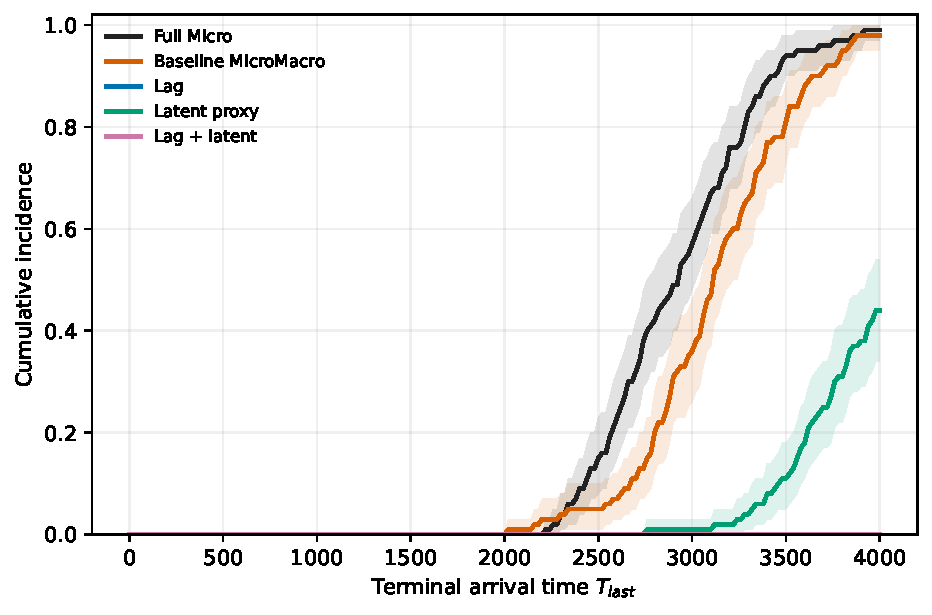
\includegraphics[width=.78\linewidth]{figures/figure_1.pdf}
\caption{Baseline cumulative incidence of terminal arrival. Curves retain all runs
and terminate at the observed completion probability; bands are pointwise 95\%
replication-bootstrap intervals.}\end{figure}
\begin{figure}[H]\centering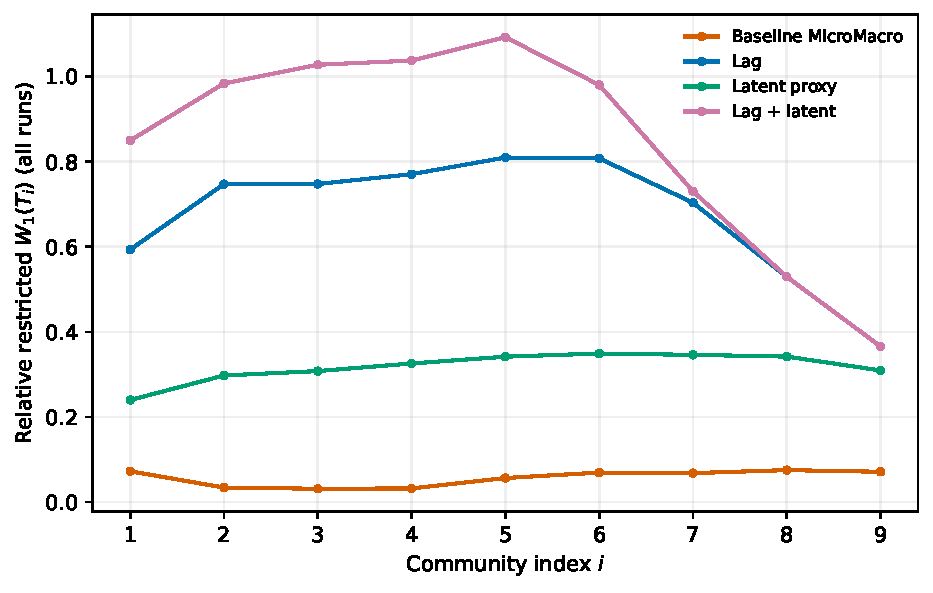
\includegraphics[width=.78\linewidth]{figures/figure_2.pdf}
\caption{Layer-wise all-run restricted relative $W_1(T_i)$ against V0. Censored
arrivals retain the common administrative horizon.}\end{figure}
\begin{figure}[H]\centering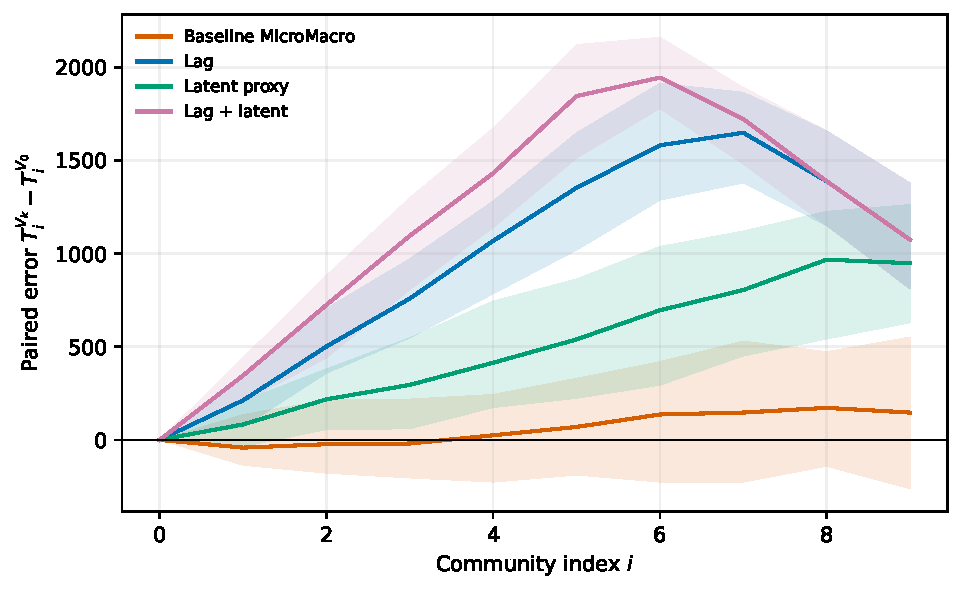
\includegraphics[width=.78\linewidth]{figures/figure_3.pdf}
\caption{Paired cumulative arrival error (variant minus V0), median and IQR over
replications; censored arrivals retain the common horizon.}\end{figure}
\begin{figure}[H]\centering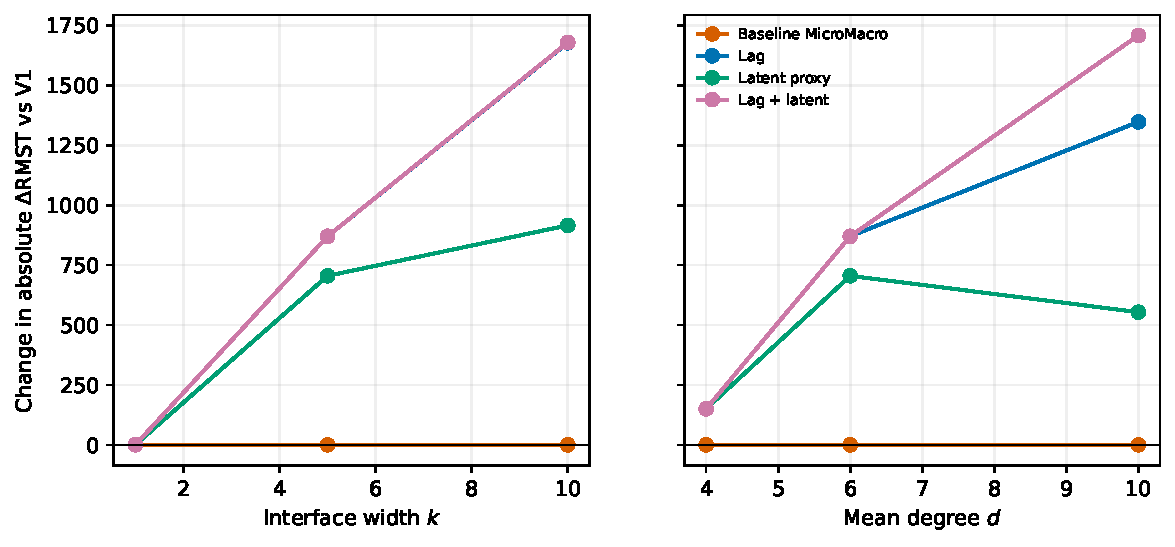
\includegraphics[width=.88\linewidth]{figures/figure_4.pdf}
\caption{Change in absolute restricted timing discrepancy relative to V1 across
the interface-width and density mini-sweeps. Positive values mean that a correction
worsened the V1 discrepancy. Baseline supplies the shared $k=5,d=6$ point.}\end{figure}

\section{Uncertainty analysis}
All confidence intervals use 2000 paired bootstrap resamples of
replication IDs. Event rows are never bootstrap units. Primary $W_1$ compares
the all-run horizon-restricted terminal-arrival distributions; completed-only
$W_1$ is a secondary conditional diagnostic normalized by the V0 completed mean.
$\Delta$RMST is variant minus V0 using all horizon-restricted runs. Equivalence
requires the entire $\Delta$RMST interval to lie within
$\pm0.05\,\mathrm{mean}(T_{last}^{V0})$.

\section{Scientific interpretation}
H1 is assessed by V2 versus V1, H2 by V3 versus V1, and their joint behavior by
V4. The replication-level factorial interaction $V4-V2-V3+V1$ on restricted
terminal arrival is -705.2 (95\% CI -798.1 to -608.8). Claims of improvement require both passed
gates and the reported uncertainty intervals; an interval containing zero alone
is not evidence of equivalence. Because several terminal cells saturate at the
administrative horizon, the terminal interaction is descriptive rather than a
clean additivity test. In the prespecified baseline sample, V1 completed in 98\% of runs and was later than V0 by $\Delta\mathrm{RMST}=200.6$ (95\% CI 98.16 to 314.6). V2 and V4 had zero terminal completions and all-run $\Delta$RMST values 1071 and 1071. V3 completed in 44\% and had $\Delta\mathrm{RMST}=905.8$. All literal corrections therefore increased delay relative to V1 and reduced completion. The same direction holds in the informative d10 and k10 sweeps. At d4 and k1, heavy censoring makes completed-only distribution metrics and apparent RMST equivalence non-diagnostic. Across the five tested cells, the literal spectral-lag and latent-proxy formulas systematically over-correct the baseline timing discrepancy.

\section{What the experiment can identify}
It can estimate relative bias reduction in the sparse baseline, distinguish H1
from H2 within the factorial cells, assess their interaction, and describe limited
scaling across the specified $d$ and $k$ values.

\section{What the experiment cannot identify}
It cannot identify recovery effects, synchronization-interval effects, placement
effects, generalization beyond connected ER communities, or computational speedup.
Runtime is an implementation diagnostic only.

\section{Limitations}
Lag may interact with midpoint hazard integration, and latent relaxation may
interact with the exponential-clock residual update. The spectral formula is a
candidate scaling law over a small descriptor range. Completed-only Wasserstein
statistics condition on arrival and therefore must be read beside completion and
all-run RMST. They are not used to claim improvement when completion probabilities
are low or materially different. V1 uses the production-aligned experimental
scheduler; the formula gates establish identity among experimental scheduler
variants, not direct pathwise identity with the production orchestrator. The $k$
and $d$ mini-sweeps are one-factor-at-a-time and do not identify an interaction or
a general scaling law.

\section{Unresolved questions}
The current design does not determine whether any remaining discrepancy is caused
by synchronization timing, placement, or non-ER boundary geometry.

\section{Recommended next experiment}
No recommendation is made outside the staged Experiment 05 evidence. Any follow-up
specified here after validation must preserve pairing and separately vary only one
previously fixed mechanism.

\section{Exact reproduction commands}
\begin{verbatim}
python -m two_layer_ctmc.experiments.experiment_05_spectral_corrections.cli \
  --stage smoke --scenario baseline --replications 5 --master-seed 270000
python -m two_layer_ctmc.experiments.experiment_05_spectral_corrections.cli \
  --stage validation --scenario all --replications 20 --resume --master-seed 270000
# Run only after explicit approval:
python -m two_layer_ctmc.experiments.experiment_05_spectral_corrections.cli \
  --stage final --scenario all --replications 100 --resume \
  --validation-approved --master-seed 270000
\end{verbatim}
\end{document}
